
\section{Auswertung}
\label{sec:Auswertung}
\subsection{Die Durchlasskurven beider LC-Ketten}
Zunächst werden die Durchlasskurven der Ketten, welche mit dem XY-Schreiber
 erstellt worden untersucht. Man beschränkt sich dabei auf die Frequenzen der
  markanten Stellen, welche die Grenzfrequenzen der Dispersionsgleichung
	 markieren. Es folgt nun zunächst die einfache $LC$-Kette:

   \begin{figure}[H]
   	\centering
   	\caption{Die Durchlasskurve der $LC$-Kette.}
   	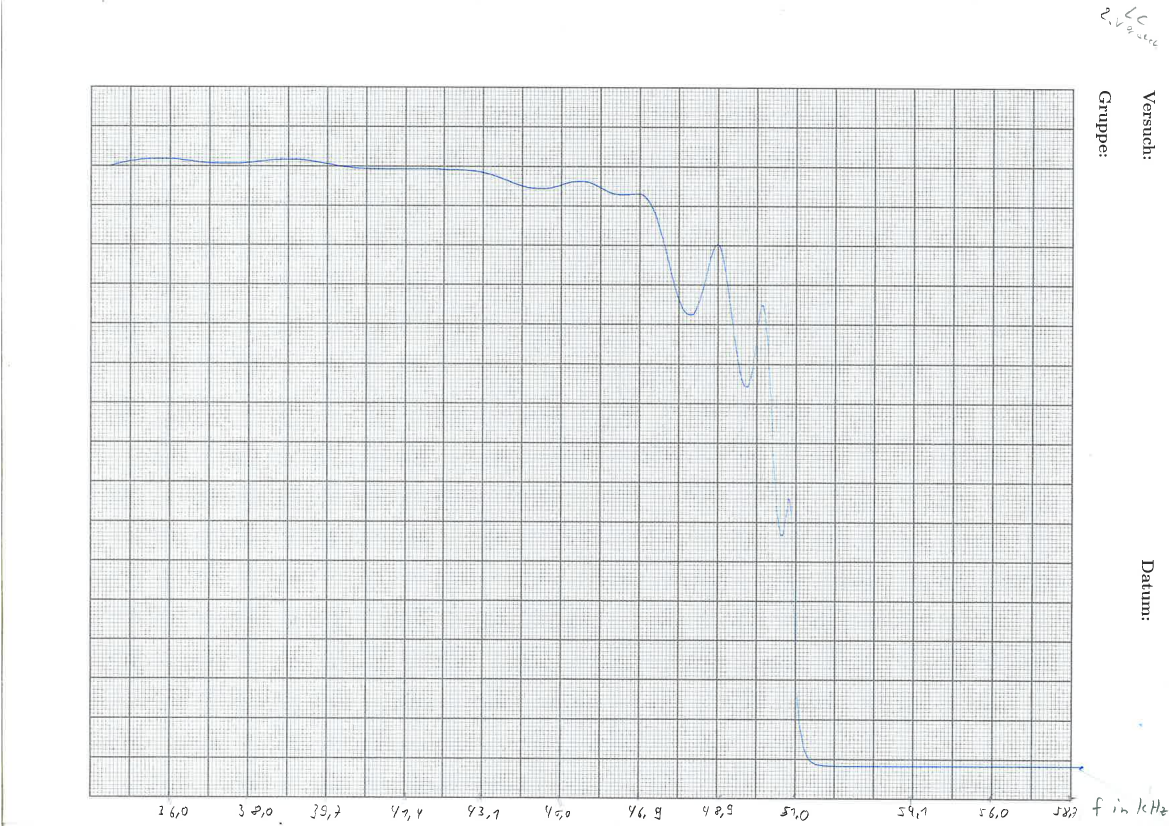
\includegraphics[width=\linewidth-70pt,height=\textheight-70pt,keepaspectratio]{content/Scans/LC.png}
   	\label{fig:Lc}
   \end{figure}

	 Für diese verschwinden, dem Ausdruck nach, sämtliche Spannungen ab ca.
	  $\SI{51}{\kilo\hertz}$. Die berechnete Grenzfrequenz liegt nach (4) bei
		 ca. $\SI{51,3}{\kilo\hertz}$. Daher liegt der bekannte Fehler bei
		  unter einem Prozent. Es folgt nun die $LC_1C_2$-Kette. Bei dieser müssen
			 sowohl die Grenzfrequenz des unteren Astes, aber auch die untere als auch obere Grenzfrequenz des
			  oberen Astes untersucht werden.

        \begin{figure}[H]
         \centering
         \caption{Die Durchlasskurve der $LC_1C_2$-Kette.}
         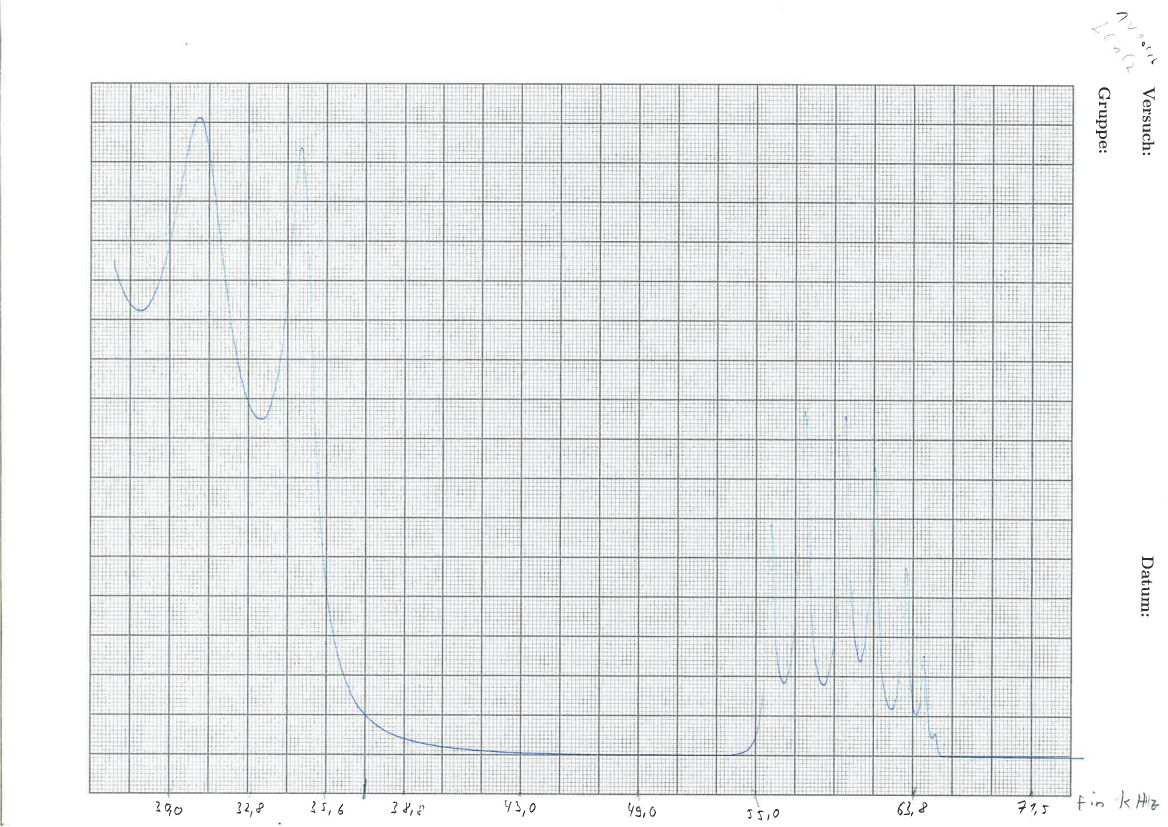
\includegraphics[width=\linewidth-70pt,height=\textheight-70pt,keepaspectratio]{content/Scans/LC1C2.png}
         \label{fig:Lc1c2}
        \end{figure}

         Aufgrund des im Graphen erkennbaren, seichten
				Ausgang am unteren Ast, lässt sich nicht genau angeben, wo die
				 Grenzfrequenz genau liegt. Sie lässt sich jedoch zwischen dem dritten
				  und dem vierten Messwert, also zwischen $\SI{35,6}{\kilo\hertz}$ und
					$\SI{38,8}{\kilo\hertz}$, vermuten, da der Graph in diesem Bereich
					 stark abflacht. Der berechnete Wert liefert ca. $\SI{36,3}{\kilo\hertz}$,
					  womit er in diesem Bereich liegt.
						 Es folgen nun die Grenzfrequenzen des oberen Astes. Die
						  untere Grenzfrequenz lässt sich am Graph bei ca. $\SI{55}{\kilo\hertz}$
							ablesen. Der berechnete Wert liegt im Gegenzug bei
							 ca. $\SI{55,5}{\kilo\hertz}$. Auch hier weicht der aus dem Graphen abgelesene Wert also nicht
							 großartig vom Theoriewert ab. Zuletzt folgt die obere Grenzfrequenz
							 des oberen Astes. Bei dieser liegt die Frequenz dem Graphen nach bei ca.
							  $\SI{65}{\kilo\hertz}$. Der Theoriewert beträgt ca. $\SI{66,3}{\kilo\hertz}$
								Auch hier passen theoretischer und experimenteller Wert zueinander.


\subsection{Die auftretende Dispersion in beiden Ketten}
\subsubsection{Die LC-Kette mit Kondensatoren einer Kapazität}
\begin{figure}[H]
	\centering
	\caption{Die Frequenz in Abhängigkeit der Phasendifferenz pro Kettenglied $LC$-Kette.}
	\includegraphics[width=\linewidth-70pt,height=\textheight-70pt,keepaspectratio]{build/grab1.pdf}
	\label{fig:grab1}
\end{figure}
\input{build/tabb1.tex}
Wie im Graph zu erkennen ist, liegen die gemessenen Werte gut auf der Theoriekurve des akustischen Astes.

\subsubsection{Die LC-Kette mit Kondensatoren zweier Kapazitäten}
\begin{figure}[H]
	\centering
	\caption{Die Frequenz in Abhängigkeit der Phasendifferenz pro Kettenglied bei einer $LC_1C_2$-Kette.}
	\includegraphics[width=\linewidth-70pt,height=\textheight-70pt,keepaspectratio]{build/grab2.pdf}
	\label{fig:grab2}
\end{figure}
\input{build/tabb2.tex}
Auch hier bestätigen die Messwerte die errechnete Theoriekurve. Hier befinden sich zusätzlich zu den Wertepaaren im akustischen Ast welche im optischen Ast und bestätigen somit dessen Existenz. 


\subsection{Bestimmung der Phasengeschwindigkeit}

\begin{figure}[H]
	\centering
	\caption{Die Phasengeschwindigkeit in Abhängigkeit der Frequenz.}
	\includegraphics[width=\linewidth-70pt,height=\textheight-70pt,keepaspectratio]{build/grac.pdf}
	\label{fig:grac}
\end{figure}
\input{build/tabc.tex}
Es zeigt sich, dass die Messwerte in der Nähe der Theoriekurve liegen und ihr Verlauf
 streng monoton fallend ist. Es sind keine größeren Abweichungen erkennbar. Am
  Verlauf der Theoriekurve lässt sich zudem wieder erkennen, dass sich, wie bereits zuvor
 gezeigt, keine Schwingungen oberhalb von ca. $\SI{51}{\kilo\hertz}$ bilden.

\subsection{Die Spannungsverläufe über eine offene LC-Kette}
\subsubsection{Für die erste Eigenschwingung}
\begin{figure}[H]
	\centering
	\caption{Der Spannungsverlauf über die offene $LC$-Kette für die 1. Eigenschwingung.}
	\includegraphics[width=\linewidth-70pt,height=\textheight-70pt,keepaspectratio]{build/grad1.pdf}
	\label{fig:grad1}
\end{figure}
Wie im Graph zu erkennen ist, bildet sich auf der $LC$-Kette eine stehende Welle aus.
 Da eine offene Kette gewählt wurde, ist die Phasendifferenz ein Vielfaches
  von $\pi$, bei der ersten 1. Eigenschwingung einfach nur $\pi$. Aufgrunddessen zeigt
 sich an beiden Enden ein Bauch,in der Mitte ein Knoten. Dies Bäuche zeigen
  den Phasensprung von $\pi$. Damit erfüllen die Messdaten die
theoretischen Überlegungen.
\subsubsection{Für die zweite Eigenschwingung}
\begin{figure}[H]
	\centering
	\caption{Der Spannungsverlauf über die offene $LC$-Kette für die 2. Eigenschwingung.}
	\includegraphics[width=\linewidth-70pt,height=\textheight-70pt,keepaspectratio]{build/grad2.pdf}
	\label{fig:grad2}
\end{figure}
Auch hier bildet die Form der Messwertkurve den Verlauf einer stehenden Welle ab.
 Diesmal jedoch den Verlauf der 2. Eigenschwingung, welcher zwei erkennbare Knoten statt einem besitzt.

\subsection{Der Spannungsverlauf auf der LC-Kette mit dem Wellenwiderstand als Abschlusswiderstand}
\begin{figure}[H]
	\centering
	\caption{Der Spannungsverlauf über die $LC$-Kette mit eingestelltem Wellenwiderstand.}
	\includegraphics[width=\linewidth-70pt,height=\textheight-70pt,keepaspectratio]{build/grad3.pdf}
	\label{fig:grad3}
\end{figure}
\input{build/tabd.tex}
Da der Wellenwiderstand für die Abschlusswiderstände eingestellt worden ist,
verhält sich die LC-Kette wie eine unendliche LC-Kette. Da diese verständlicherweise
 kein Ende besitzt, an dem eine Reflexion geschehen könnte, bildet sich keine stehende Welle aus.
  Daher bleibt der Spannungsverlauf des Graphen konstant. Die Messwerte
   bestätigen also die Theoriekurve.
